
\chapter{File and Folder Structure}
\label{cha:file-fold-struct}

\section{ABD Folder}
\label{sec:abd-folder}

To compile the HOL code in this project, open a command line prompt in the HOL folder and do the following.
\begin{itemize}
  \item execute "Holmake cleanAll"
\item execute "make clean"
\item execute "Holmake"
\item execute "make"
\end{itemize}

ABD was the Assured by Design folder.  At the time of this document, there were two subfolders in the ABD
folder: PatrolBase and UAV.  The PatrolBase folder contained the work performed on this project and described
in this documentation.  The UAV folder contained other ABD work that were not covered in this project.
The UAV work was not discussed in this documentation.  (Note that all references to \emph{this project}
refer only to the patrol base portion of the ABD project.)\\

 \begin{figure}[h]
  \centering
  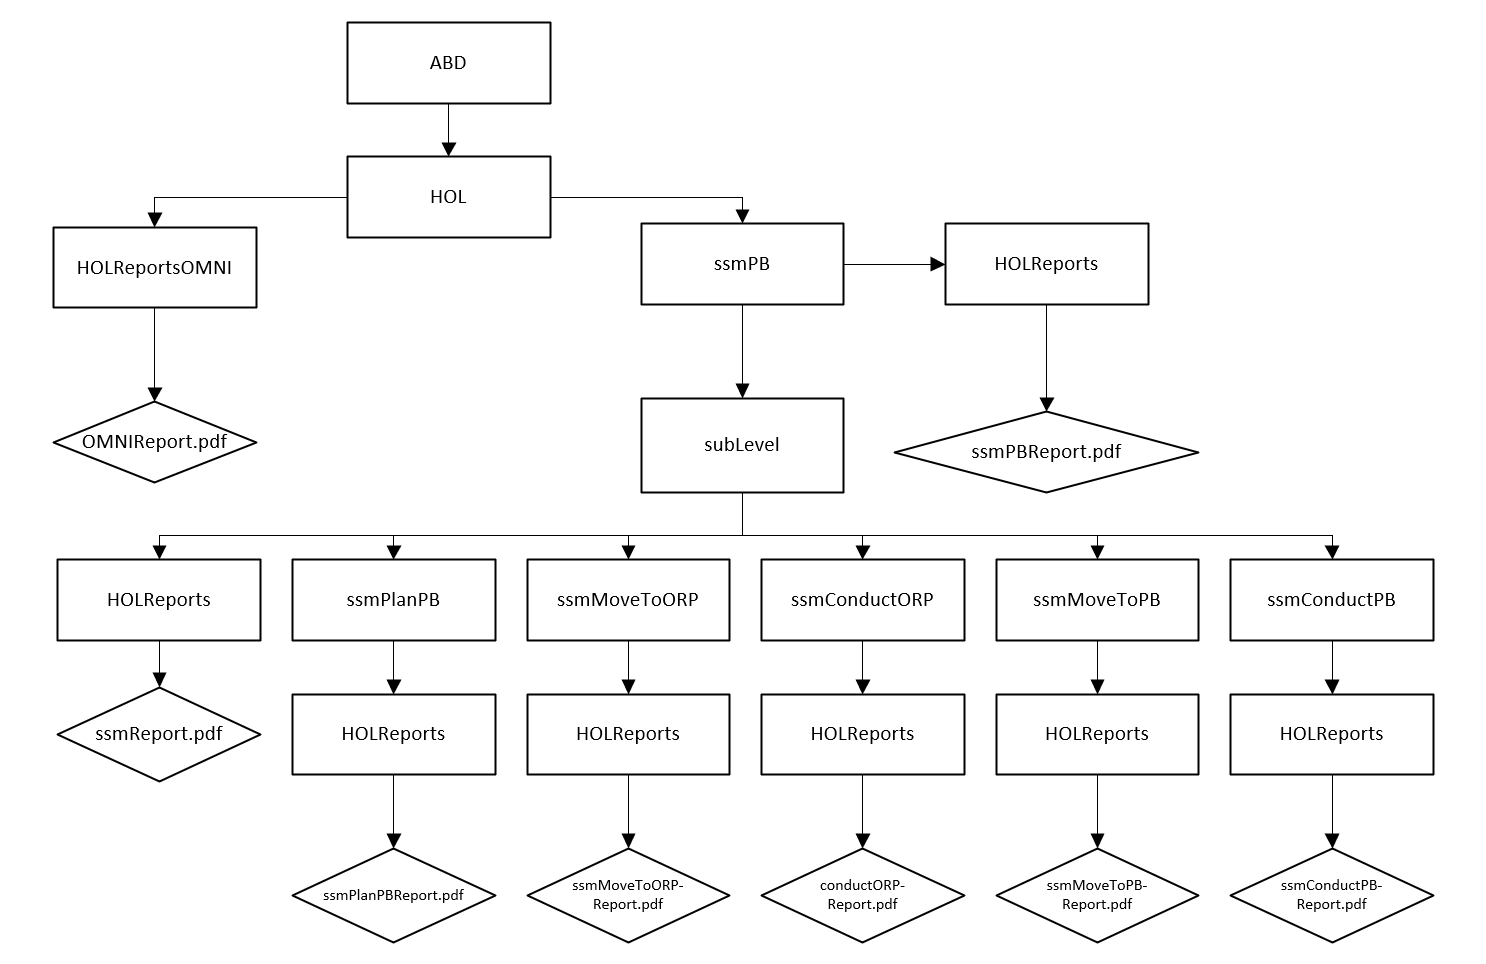
\includegraphics[width=0.8\linewidth]{ABDfolder.PNG}
  \caption{ABD Folder Structure}
\end{figure}

The overall layout of the ABD folder was shown in figure 2.1.   HOL contained the HOL code and EmitTeX
reports for the translation of the patrol base operations into \emph{secure} state machines.  The Word
folder, at the time of this documentation, was empty and in the future will contain a conversion of this
documentation into Word format.  The LaTeX folder contained the LaTeX formatted documentation for this
project.  The PBTranslations folder contained the subject matter expert's diagrams which were translations
of the Ranger Manual into the hierarchy of secure state machines.

 

\section{Word}
\label{sec:word}

This folder contained this documentation in Word format.

\section{PBTranslations}
\label{sec:pbtranslations}

This folder contained the subject matter expert's diagrams which were translations of the ranger manual
into the hierarchy of secure state machines.

\section{LaTeX}
\label{sec:latex}

This folder contained the LaTeX formatted documentation for the patrol base project.\\

Figure 2.2 showed the LaTeX folder structure. The LaTeX folder contained all the files that were used to generate this documentation. This documentation was generated by using the book class of LaTeX, which there was a master file that was linked to several other files that contained the contents for each portion of the documentation. This class allowed us to separate the contents of this entire documentation into several smaller files, and it also enabled us to create a book structure of parts followed with chapters, sections, subsections, and subsubsections. \\

The master file of this documentation was called PatrolBaseDoc.tex, which it resided in the LaTeX directory. This master file does not contain any content for this documentation; it simply acted as the backbone with paths linked to the files that contained the contents for this documentation. It also called for all the necessary LaTeX packages used to generate this report. \\

The content files for each part of this report resided in their dedicated subdirectories, which are the folders that the LaTeX top directory points to in Figure 2.2. The files responsible for the Preface, Acknowledgments, Summary, Introduction, Future Works and Research, Conclusions, Recommendations, Appendices, and References chapters of this report were in the preface, acknowledgments, summary, Intro, futureWorks, conclusion, recommendations, appendix, and references subdirectories respectively. For the Results and Results and Discussion for ACL and HOL Verification parts and their chapters were all in the MethodsAP and HOLImplementation subdirectories.\\

Some of these subdirectories also contained a picture folder, and it contained all the images used in this documentation. 
\begin{figure}[h]
  \centering
  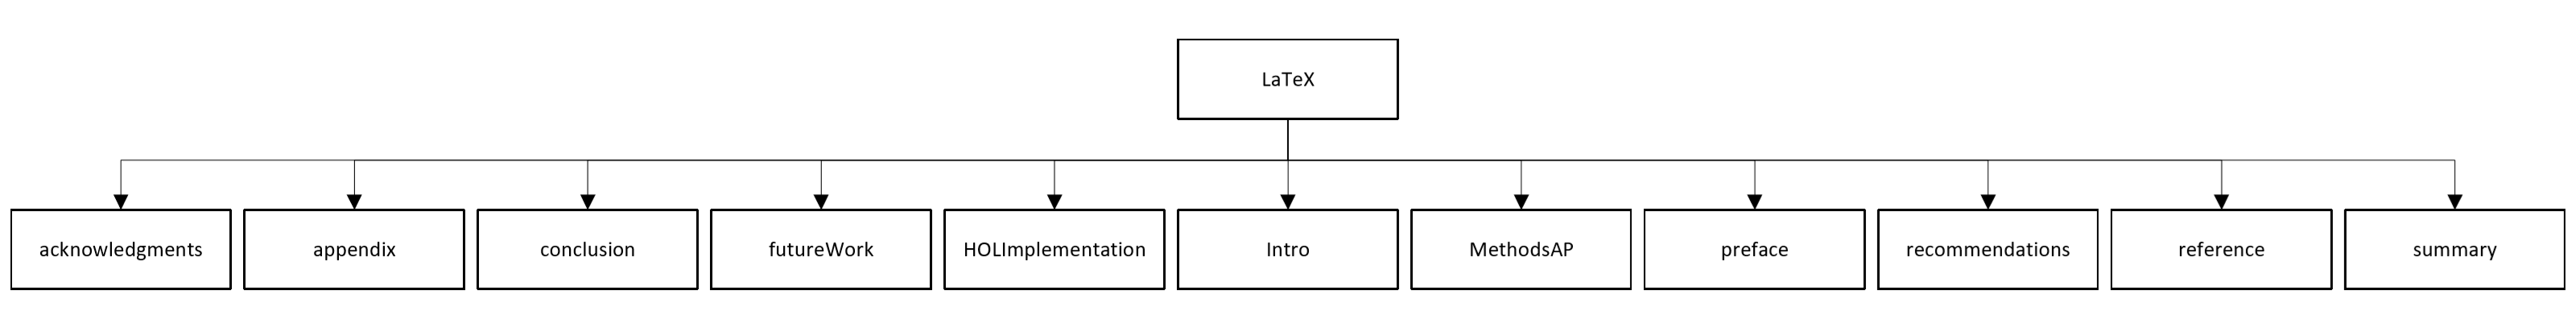
\includegraphics[width=1\linewidth]{LatexFolderStructure.PNG}
  \caption{LaTeX Folder Structure}
\end{figure}

\section{HOL}
\label{sec:hol}

Figure 2.3  showed the OMNI-level folder.  OMNI-level contained the files and folders that were used by the entire project. Definitions for datatypes used in ALL \emph{secure} state machines were coded in OMNITypeScript.sml.  The parameterizable \emph{secure} state machines were defined in ssm11 and ssm.  Theories needed for ssm11 and ssm to work were defined in satListScript.sml, ssminfRules.sig, and ssminfRules.sml.  The Holmakefile file was included in all folders.  This file told Holmake where to find the theory files needed to run Holmake. 

\begin{figure}[h]
  \centering
  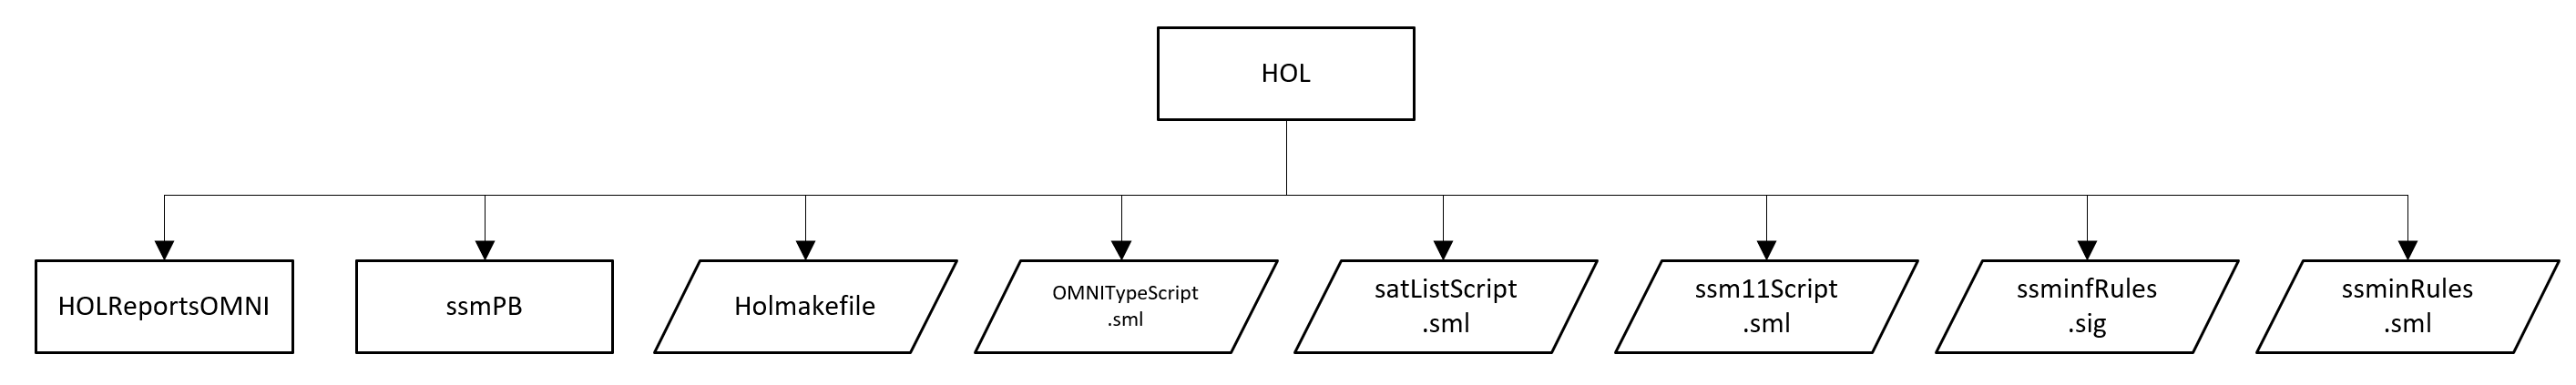
\includegraphics[width=1\linewidth]{HOLOMNI.PNG}
  \caption{HOL OMNI-level Folder}
\end{figure}

\subsection{HOLReports}
\label{sec:holreports}

HOLReports was defined as a subfolder in each folder containing a \emph{secure} state machine. These folders contained the documentation for the theories in this project.  The HOLReports folder for the OMNI-level was named HOLReportsOMNI.  It was named differently than the other HOLReports folders because it contained documentation for all the theories in the project, whereas the other HOLReports folders contained documentation for only the theories for which they were a subfolder.\\

Figure 2.4  showed the contents of a typical HOLReports folder. The HOLReports folders contained the files needed to generate the EmitTeX pretty-printed pdf files for the HOL theories.  EmitTeX converted the datatypes, definitions, and theorems in the *Script.sml files into pretty-printed text and saved the results in *Report.pdf.  For HOLReportsOMNI, the documentation was saved in OMNIReport.pdf.  A copy of OMNIReport.pdf was included in the \hyperlink{OMNIReport}{appendix H}.  The documentation can be generated for the theories by doing the following from within any HOLReports folder. 

\begin{itemize}
  \item At the command line, 
\item execute "Holmake cleanAll"
\item execute "make clean"
\item execute "Holmake"
\item execute "make"
  \end{itemize}

\begin{figure}[h]
  \centering
  \includegraphics[width=1\linewidth]{HOLReport.PNG}
  \caption{HOLReports}
\end{figure}

\subsubsection{Documentation.sml}
\label{sec:documentation.sml}

documentation.sml loaded EmitTeX and the required *Script.sml files into HOL.  It then opened EmitTeX and applied the print_theories_as_tex_doc function on the *Script.sml files.

\subsubsection{holtex.sty and holtexbasic.sty}
\label{sec:holt-holt}

holtex.sty and holtexbasic. sty were style files that told HOL how to format the HOLReport.pdf file generated by EmitTeX.

\subsubsection{Makefile}
\label{sec:makefile}

Makefile told the command prompt to send documentation.sml to Holmake.  It then instructed HOL to produce the pdf report using PDFLATEX and MAKEINDEX.

\subsection{ssmPB}
\label{sec:ssmpb}


Figure 2.5 showed the files and folders in ssmPB.  This was the top-level \emph{secure} state machine.  It contained two theories: PBTypeScript.sml and ssmPBScript.sml.  PBTypeScript.sml contained the type definitions for this \emph{secure} state machine.  ssmPBScript.sml contained the code for this \emph{secure} state machine.  

\begin{figure}[h]
  \centering
  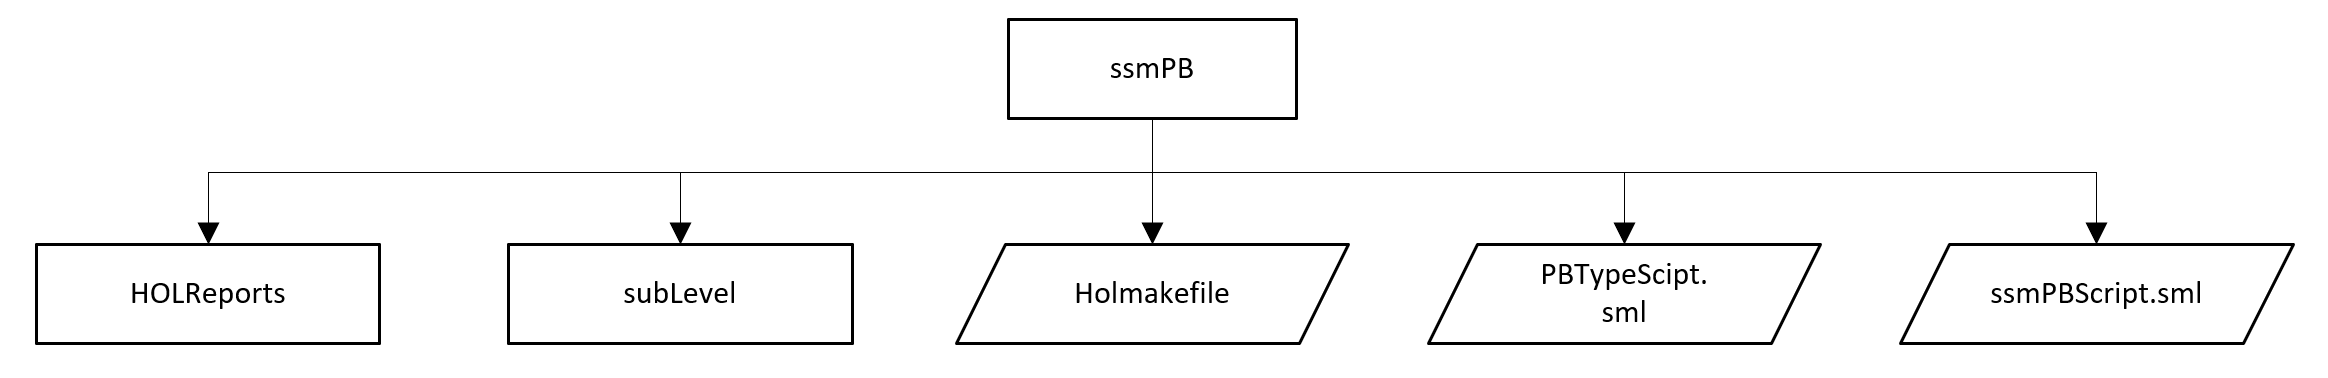
\includegraphics[width=1\linewidth]{ssmPB.PNG}
  \caption{ssmPB, Example of a Secure State Machine Folder}
\end{figure}

\subsection{subLevel}
\label{sec:sublevel}
The subLevel folder was found in the ssmPB folder.  The subLevel folder contained the folders for the sub-level \emph{secure} state machines.  The contents were similar to ssmPB, one *TypeScript.sml file and one ssm*Script.sml file for each sub-level subfolder.

\subsection{Additional Folders}
\label{sec:additional-folders}

Additional folders were planned as needed as the project progresses.









% ---- this points LaTeX to PatrolBaseDoc.tex ----
% Local Variables:
% TeX-master: "../PatrolBaseDoc"
% End: